% DSC 261 final report. Built on the PVLDB template (acmart v2.19) used for the proposal.
% Numbers come from generated/numbers.tex and tables from generated/*.tex, both written by
%   python make_report_assets.py --run runs/full --dest report
% so the text cannot drift from the data. Items marked \todo are finalized after the full run.

\documentclass[sigconf, nonacm]{acmart}

%%% VLDB block start %%%
\usepackage{pvldb}
%%% VLDB block end %%%
\usepackage{booktabs}
\usepackage{xcolor}

\renewcommand\vldbdoi{XX.XX/XXX.XX}
\renewcommand\vldbpages{XXX-XXX}
\renewcommand\vldbavailabilityurl{}

\newcommand{\todo}[1]{\textcolor{red}{[TODO: #1]}}
\setlength{\emergencystretch}{1.5em}
\renewcommand{\topfraction}{0.9}\renewcommand{\dbltopfraction}{0.9}
\renewcommand{\textfraction}{0.07}\renewcommand{\floatpagefraction}{0.75}
\renewcommand{\dblfloatpagefraction}{0.75}
\InputIfFileExists{generated/numbers.tex}{}{}
\providecommand{\BaseAcc}{\todo{n}}\providecommand{\BaseTPR}{\todo{n}}\providecommand{\BaseFPR}{\todo{n}}
\providecommand{\BasePSNR}{\todo{n}}\providecommand{\RunDevice}{\todo{GPU}}
\providecommand{\RunEpochs}{10}\providecommand{\RunHours}{\todo{n}}
\makeatletter
\@for\wm@a:={Fgsm,Pgd,Noise}\do{\@for\wm@m:={Acc,Asr,Tpr,Fpr,Psnr}\do{\@for\wm@t:={A,B,C,D,E}\do{%
  \expandafter\providecommand\csname Base\wm@a\wm@m\wm@t\endcsname{\todo{n}}}}}
\makeatother

\begin{document}
\title{Robustness of Vision Watermark Detection Against Adversarial Attacks}
\subtitle{DSC 261 Final Report}

\author{Emily Cheng}\affiliation{\institution{}\city{}\state{}\country{}}\email{emc027@ucsd.edu}
\author{Seongho Kim}\affiliation{\institution{}\city{}\state{}\country{}}\email{sek065@ucsd.edu}
\author{Paul Lai}\affiliation{\institution{}\city{}\state{}\country{}}\email{holai@ucsd.edu}
\author{Kevin Lin}\affiliation{\institution{}\city{}\state{}\country{}}\email{kel100@ucsd.edu}
\author{Samantha Lin}\affiliation{\institution{}\city{}\state{}\country{}}\email{yul186@ucsd.edu}
\author{Ariel Wang}\affiliation{\institution{}\city{}\state{}\country{}}\email{juw115@ucsd.edu}

\begin{abstract}
Invisible watermarks are a leading proposal for labelling AI-generated images, and they are
increasingly checked by learned detectors. We study how easily such a detector can be fooled.
We embed a fixed pseudorandom $\pm\lambda$ pattern into CIFAR-10 images and fine-tune an
ImageNet-pretrained ResNet50 to tell watermarked from unwatermarked images. The detector is
accurate on unmodified images (\BaseAcc\% accuracy at $\lambda=0.02$, PSNR \BasePSNR\,dB). We then
attack it with FGSM and PGD at $L_\infty$ budgets from $0.0025$ to $0.03$, train FGSM- and
PGD-adversarially-trained detectors, and vary the watermark strength $\lambda$. We also prove a
simple limit: once the attack budget reaches $\lambda/2$, no detector of any kind can classify
both the clean and the watermarked copy of an image correctly, so accuracy on a balanced
paired test set is capped at 50\%. The experiments match this limit. PGD perturbations far smaller
than the watermark evade most detections (\BasePgdAsrB\% at $\epsilon=\lambda/4$), and PGD beats
FGSM everywhere; FGSM fails at large budgets because the detector treats any dense noise as a
watermark. PGD adversarial training cuts PGD's evasion rate at $\lambda/4$ from \BasePgdAsrB\% to
\PatAPgdAsrB\%, but no detector survives past $\lambda/2$, and a stronger watermark buys robustness
only by lowering fidelity. An additive watermark's robustness is set by its own amplitude.
\end{abstract}

\maketitle

\section{Introduction}
Generative models make it hard to tell authentic images from synthetic or manipulated ones,
which raises concerns about misinformation, copyright, and provenance. Invisible watermarking
addresses this by embedding an identifying signal that leaves the image visually unchanged but
can be recovered by a detector~\cite{paper4,paper5,paper6}. A watermark is only useful if the
detector still finds it after the image has been modified, including by someone who wants it gone.

Neural networks are known to be vulnerable to adversarial examples: small, deliberately chosen
pixel changes that flip their predictions~\cite{paper7,paper2}. A neural watermark detector
should therefore be vulnerable too. In this project we measure how vulnerable, and whether
adversarial training~\cite{paper3} fixes it. Our hypotheses, stated in the proposal, were:
\begin{description}
  \item[H1] Detection accuracy falls as the attack budget $\epsilon$ grows.
  \item[H2] PGD, being iterative, evades detection more effectively than single-step FGSM.
  \item[H3] Adversarially trained detectors resist attacks better than a standard detector.
  \item[H4] A stronger watermark (larger $\lambda$) is more robust but lowers image fidelity.
\end{description}
\noindent Our contributions are (i) a complete, reproducible evaluation of all four hypotheses on
a paired test set; (ii) a short proof that robust detection of an additive $\pm\lambda$ watermark
is impossible for $\epsilon \ge \lambda/2$, which explains where adversarial training must fail;
and (iii) measurements of the attacks' cost in image quality (PSNR, SSIM).

\section{Related Work}
\textbf{Deep learning based watermarking.} Zhu et al.\ introduced HiDDeN, showing that neural
networks can learn to encode and recover hidden information in images and studying robustness to
cropping, blurring, and JPEG compression~\cite{paper4}.

\textbf{Watermarking generated images.} Tree-Ring watermarks embed a pattern in the initial noise
of a diffusion model~\cite{paper5}; Stable Signature fine-tunes a latent diffusion decoder so that
every output carries a recoverable signature~\cite{paper6}. Both stress robustness to image edits.

\textbf{Adversarial attacks and defenses.} Szegedy et al.\ first described adversarial
examples~\cite{paper7}. Goodfellow et al.\ proposed FGSM~\cite{paper2}; Madry et al.\ framed
robustness as min-max optimization, attacked with PGD, and trained against it~\cite{paper3}.
Wong et al.\ showed that FGSM-based adversarial training can suffer ``catastrophic overfitting'',
becoming robust to FGSM but not PGD~\cite{wong2020fast}.

\textbf{Residual networks.} ResNet's residual connections make deep networks trainable~\cite{paper1};
we use ResNet50 as the detector.

Unlike these works, we do not propose a watermark. We use a deliberately simple fixed-pattern
watermark as a controlled baseline and systematically measure how a learned detector for it
fails under gradient attacks, and why.

\section{Method}
\subsection{Data}
We use CIFAR-10~\cite{cifar10}: 50{,}000 training and 10{,}000 test RGB images of size
$32\times32$ in ten classes. Pixel values are scaled to $[0,1]$. Original images are split
\emph{before} watermarking so that no source image appears in two partitions: 45{,}000 training
and 5{,}000 validation originals (stratified by class), and the 10{,}000 test originals. In the
training and validation sets exactly half of each class is watermarked (label 1) and the rest is
left clean (label 0).

For testing we use a \emph{paired} design, as proposed: every test original appears twice, once
clean and once watermarked, giving 20{,}000 test images. This makes the test set exactly
balanced and lets us compare the two versions of the same image directly.

\subsection{Watermark}
Let $x \in [0,1]^{3\times32\times32}$ be an image and $W \in \{-1,+1\}^{3\times32\times32}$ a fixed
pseudorandom pattern (seed 2026). The watermarked image is
\[ x_W = \operatorname{clip}_{[0,1]}(x + \lambda W). \]
$\lambda$ sets the strength. Our main experiments use $\lambda = 0.02$ (about $5/255$), which
gives a mean PSNR of \BasePSNR\,dB on the test set; the strength study uses
$\lambda \in \{0.005, 0.01, 0.02, 0.05\}$.

\subsection{Detector}
The detector is an ImageNet-pretrained ResNet50 (torchvision's V2 weights) whose
1000-way classification layer is replaced by a 2-way layer. It takes $32\times32$ inputs
directly. ImageNet mean/std normalization is implemented as the model's first layer, so attacks
operate on, and budgets are measured in, ordinary $[0,1]$ pixel units.

\subsection{FGSM attack}
FGSM~\cite{paper2} takes one step of size $\epsilon$ in the direction that increases the loss:
\[ x_{\text{adv}} = \operatorname{clip}_{[0,1]}\big(x + \epsilon\,\operatorname{sign}(\nabla_x L(f_\theta(x), y))\big), \]
where $L$ is cross-entropy and $y$ the true label. On a watermarked image this pushes the
detector toward ``clean'' (evasion); on a clean image, toward ``watermarked'' (forgery).

\subsection{PGD attack}
PGD~\cite{paper3} iterates smaller signed-gradient steps and projects back onto the allowed region:
\[ x^{t+1} = \Pi_{B_\epsilon(x)\cap[0,1]^d}\big(x^t + \alpha\,\operatorname{sign}(\nabla_{x^t} L(f_\theta(x^t), y))\big), \]
with $B_\epsilon(x)$ the $L_\infty$ ball of radius $\epsilon$. We use 10 steps of size
$\alpha=\epsilon/4$ from a uniform random start in $B_\epsilon(x)$, so the iterate can travel
$2.5\epsilon$ and reach any point of the ball.

\subsection{Adversarial training}
Adversarial training replaces part of each training batch with attacked images. Following the
mixed objective of~\cite{paper2}, every step trains on a clean batch concatenated with its
adversarial version (FGSM or PGD, generated on the fly against the current model). We train FGSM-
and PGD-trained detectors at $\epsilon_{\text{train}} \in \{0.005, 0.01\}$, i.e.\ $\lambda/4$ and
$\lambda/2$; Section~\ref{sec:limit} explains why larger training budgets cannot work.

\subsection{A limit on robust detection}\label{sec:limit}
\textbf{Proposition.} Let $x_0\in[0,1]^d$ and $x_1 = \operatorname{clip}(x_0 + \lambda W)$ with
$W\in\{\pm1\}^d$. If $\epsilon \ge \lambda/2$, then for \emph{every} detector $f$ at least one of
$x_0, x_1$ can be moved, within an $L_\infty$ budget $\epsilon$, to a point that $f$ misclassifies.

\emph{Proof.} Let $z = (x_0 + x_1)/2$. Clipping can only shrink a coordinate's change, so
$|x_1 - x_0| \le \lambda$ coordinatewise, hence $\|z - x_0\|_\infty \le \lambda/2 \le \epsilon$ and
$\|z - x_1\|_\infty \le \epsilon$; $z\in[0,1]^d$ because it is an average of two valid images.
$f(z)$ is a single label. If $f(z)=1$, the clean copy moved to $z$ is misclassified; if $f(z)=0$,
the watermarked copy moved to $z$ is. \hfill$\square$

\noindent Consequently, against an optimal attacker on our paired test set, the fraction of
originals whose two versions are \emph{both} classified correctly is $0$, and accuracy is at most
$50\%$. For $\epsilon \ge \lambda$ the situation is stronger: an evader can subtract the watermark
entirely ($z = x_0$), so a watermarked image becomes literally identical to the original and the
detection rate can be driven down to the detector's false-positive rate. These are
information-theoretic limits: they hold for any model, architecture, or training method, and
adversarial training can only help below $\lambda/2$.

\subsection{Evaluation protocol}
For each detector we report, on the paired test set, accuracy, true-positive rate (TPR,
watermarked images detected), false-positive rate (FPR, clean images flagged), and precision,
both on unmodified images and under each attack. Following the proposal, the \emph{evasion attack
success rate} (ASR) is the fraction of watermarked images that the detector caught before the
attack and misses after it. We also report the \emph{forgery} ASR (clean images correctly cleared
before the attack and flagged after it), the paired accuracy (both versions of an original
correct), and image quality of each attacked image relative to its unattacked input: PSNR and
SSIM~\cite{wang2004ssim}. As a non-adversarial control we also add \emph{random} $\pm\epsilon$
sign noise (each pixel independently $\pm\epsilon$), which has the same size and structure as an
FGSM perturbation but no information about the model. Attacks are white-box: the attacker knows the model but not $W$
explicitly. Budgets are $\epsilon \in \{0.0025, 0.005, 0.01, 0.02, 0.03\}$, which bracket
$\lambda/2$ and $\lambda$ for every $\lambda$ studied.

\section{Experimental Setup}
\begin{table}[t]
\caption{Training and evaluation settings.}\label{tab:setup}
\small
\begin{tabular}{ll}
\toprule
Optimizer & SGD, lr $10^{-3}$, momentum 0.9 \\
Batch size & 128 (256 incl.\ adversarial half) \\
Epochs & \RunEpochs; keep best validation epoch$^{*}$ \\
Precision & mixed (fp16) training; attacks in fp32 \\
PGD & 10 steps, $\alpha=\epsilon/4$, random start \\
Attack budgets & 0.0025, 0.005, 0.01, 0.02, 0.03 \\
Adv.\ training budgets & 0.005, 0.01 \\
Watermark strengths & 0.005, 0.01, 0.02, 0.05 \\
GPU & \RunDevice \\
GPU time & \RunHours\,h (all 8 detectors, training + evaluation) \\
\bottomrule
\end{tabular}\\[2pt]
{\footnotesize $^{*}$Score: clean validation accuracy (standard training) or the mean of clean and
robust validation accuracy at the training $\epsilon$ (adversarial training).}
\end{table}
Table~\ref{tab:setup} lists the settings. All models start from the same pretrained weights and
the same random head initialization (seed 0), and use identical data splits and watermark labels.
Code, logs, and per-configuration results are in the project repository.

\textbf{Changes from the proposal.} (1) The proposal's early-stopping rule compared the last
mini-batch loss across epochs, which is noisy and stopped the first baseline after 4 of 15 epochs
while validation accuracy was still rising; we instead train a fixed number of epochs and keep the
best validation epoch. (2) Adversarial training budgets are limited to $\epsilon \le \lambda/2$
because of the proposition in Section~\ref{sec:limit}. (3) PGD uses a step size tied to $\epsilon$
and a random start so that it can always use its full budget. (4) We added the forgery ASR and
paired accuracy, which the paired test design makes possible.

\section{Results}
\subsection{Detection without attacks}
\begin{table}[t]
\caption{Detection on unmodified paired test images (\%).}\label{tab:clean}
\small
\IfFileExists{generated/table_clean.tex}{\begin{tabular}{lrrrrr}
\toprule
Detector & $\lambda$ & Acc. & TPR & FPR & Prec. \\
\midrule
Standard & 0.005 & 62.0 & 59.1 & 35.1 & 62.8 \\
Standard & 0.01 & 86.4 & 87.8 & 15.0 & 85.4 \\
Standard & 0.02 & 97.7 & 98.1 & 2.7 & 97.4 \\
FGSM-AT ($\epsilon$=0.005) & 0.02 & 97.1 & 99.6 & 5.3 & 95.0 \\
FGSM-AT ($\epsilon$=0.01) & 0.02 & 96.4 & 98.5 & 5.6 & 94.6 \\
PGD-AT ($\epsilon$=0.005) & 0.02 & 94.2 & 96.5 & 8.2 & 92.2 \\
PGD-AT ($\epsilon$=0.01) & 0.02 & 86.0 & 76.3 & 4.2 & 94.7 \\
Standard & 0.05 & 99.9 & 99.9 & 0.1 & 99.9 \\
\bottomrule
\end{tabular}
}{\todo{table}}
\end{table}
The standard detector at $\lambda=0.02$ reaches \BaseAcc\% accuracy, with TPR \BaseTPR\% and FPR
\BaseFPR\% (Table~\ref{tab:clean}), up from 96.3\% for the team's first baseline, which the old
early-stopping rule halted after 4 epochs. Adversarial training costs clean accuracy, little for
FGSM training (\FatACleanAcc\% and \FatBCleanAcc\%) and more for PGD training (\PatACleanAcc\% at
$\epsilon_{\text{train}}=0.005$ and \PatBCleanAcc\% at $0.01$). Detection gets harder as the watermark
gets fainter: \LamDCleanAcc\% at $\lambda=0.05$ but only \LamACleanAcc\% at $\lambda=0.005$, a change
of about $1.3/255$ per pixel.

\subsection{H1: Accuracy falls as the budget grows}
\begin{figure*}[t]
\centering
\IfFileExists{figures/fig_h1_h2_baseline.pdf}{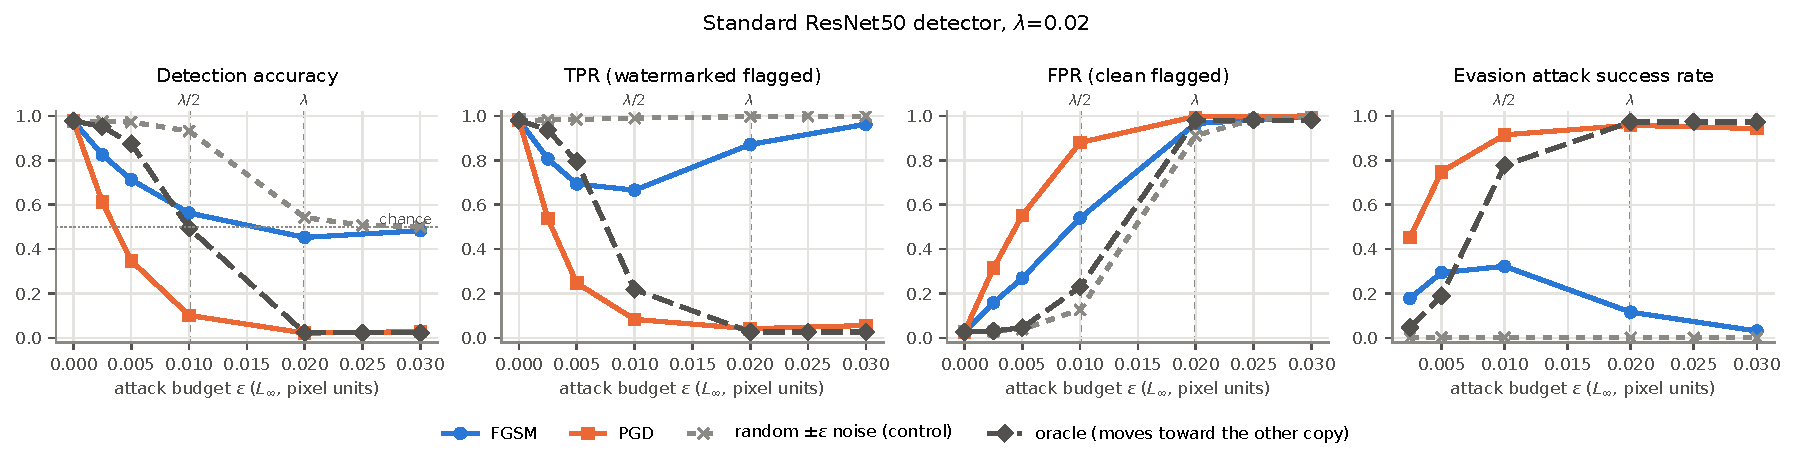
\includegraphics[width=\textwidth]{figures/fig_h1_h2_baseline.pdf}}{\todo{figure}}
\caption{Standard detector ($\lambda=0.02$) under FGSM, PGD, and random $\pm\epsilon$ sign noise
(control). Dashed lines mark $\lambda/2$, beyond which no detector can be robust, and $\lambda$,
beyond which an attacker can remove the watermark entirely. Evasion ASR: fraction of detected
watermarked images that the attack makes undetected.}
\label{fig:baseline}
\end{figure*}
Figure~\ref{fig:baseline} shows the standard detector under attack. Under PGD, accuracy falls
steadily with the budget: from \BaseAcc\% on unmodified images to \BasePgdAccA\% at
$\epsilon=0.0025$ ($\lambda/8$, a change of 0.6/255 per pixel; PSNR \BasePgdPsnrA\,dB),
\BasePgdAccB\% at $\epsilon=0.005$, \BasePgdAccC\% at $\lambda/2$, and \BasePgdAccD\% at $\lambda$,
far below chance. Under FGSM, accuracy also falls, to \BaseFgsmAccD\% at $\epsilon=\lambda$, but
then stops falling (\BaseFgsmAccE\% at $\epsilon=0.03$). \textbf{H1 holds}: for PGD at every budget,
and for FGSM up to $\epsilon\approx\lambda$.

\textbf{Why FGSM stops working: the detector responds to noise, not just to $W$.} FGSM's
turnaround is visible in the TPR and FPR panels. At $\epsilon=0.03$ FGSM makes the detector flag
\BaseFgsmFprE\% of clean images while still flagging \BaseFgsmTprE\% of watermarked ones; its
evasion success drops to \BaseFgsmAsrE\%. FGSM adds a dense $\pm\epsilon$ sign pattern to every
pixel, which is exactly the form of our watermark. Our control confirms that the detector reacts to
that form rather than only to the specific pattern $W$: adding \emph{random} $\pm\epsilon$ sign
noise, which carries no information about the model, leaves accuracy nearly unchanged for
$\epsilon\le0.005$ (\BaseNoiseAccB\%), but makes the detector flag \BaseNoiseFprC\% of clean images
at $\epsilon=0.01$, \BaseNoiseFprD\% at $0.02$, and \BaseNoiseFprE\% at $0.03$. Random noise never
removes a watermark (evasion ASR at most \BaseNoiseAsrB\% at any budget). So once the perturbation is about as
large as the watermark, a single FGSM step mostly adds watermark-like noise and the detector says
``watermarked'' regardless of the true label. This is also a practical weakness: an adversary with
no access to the model can make clean images look watermarked (a forgery or false-alarm attack)
simply by adding random noise of amplitude $\approx\lambda$.

\subsection{H2: PGD versus FGSM}
PGD is far more effective than FGSM at every budget (Figure~\ref{fig:baseline}, right). Its
evasion success rate is \BasePgdAsrA\% versus \BaseFgsmAsrA\% for FGSM at $\epsilon=0.0025$,
\BasePgdAsrB\% versus \BaseFgsmAsrB\% at $0.005$, and \BasePgdAsrC\% versus \BaseFgsmAsrC\% at
$\lambda/2$. FGSM relies on a single linear step, which the previous paragraph shows degenerates
into watermark-like noise; PGD's small iterative steps follow the detector's non-linear decision
boundary instead. \textbf{H2 holds} for every detector we trained: across all 8 detectors and 5
budgets, PGD lowers accuracy more than FGSM in 40 of 40 cases and has the higher evasion success
rate in 39 of 40 (the exception is a 0.2-point tie for PGD-AT at $\epsilon=0.005$).

\subsection{H3: Adversarial training}
\begin{figure*}[t]
\centering
\IfFileExists{figures/fig_h3_adv_training.pdf}{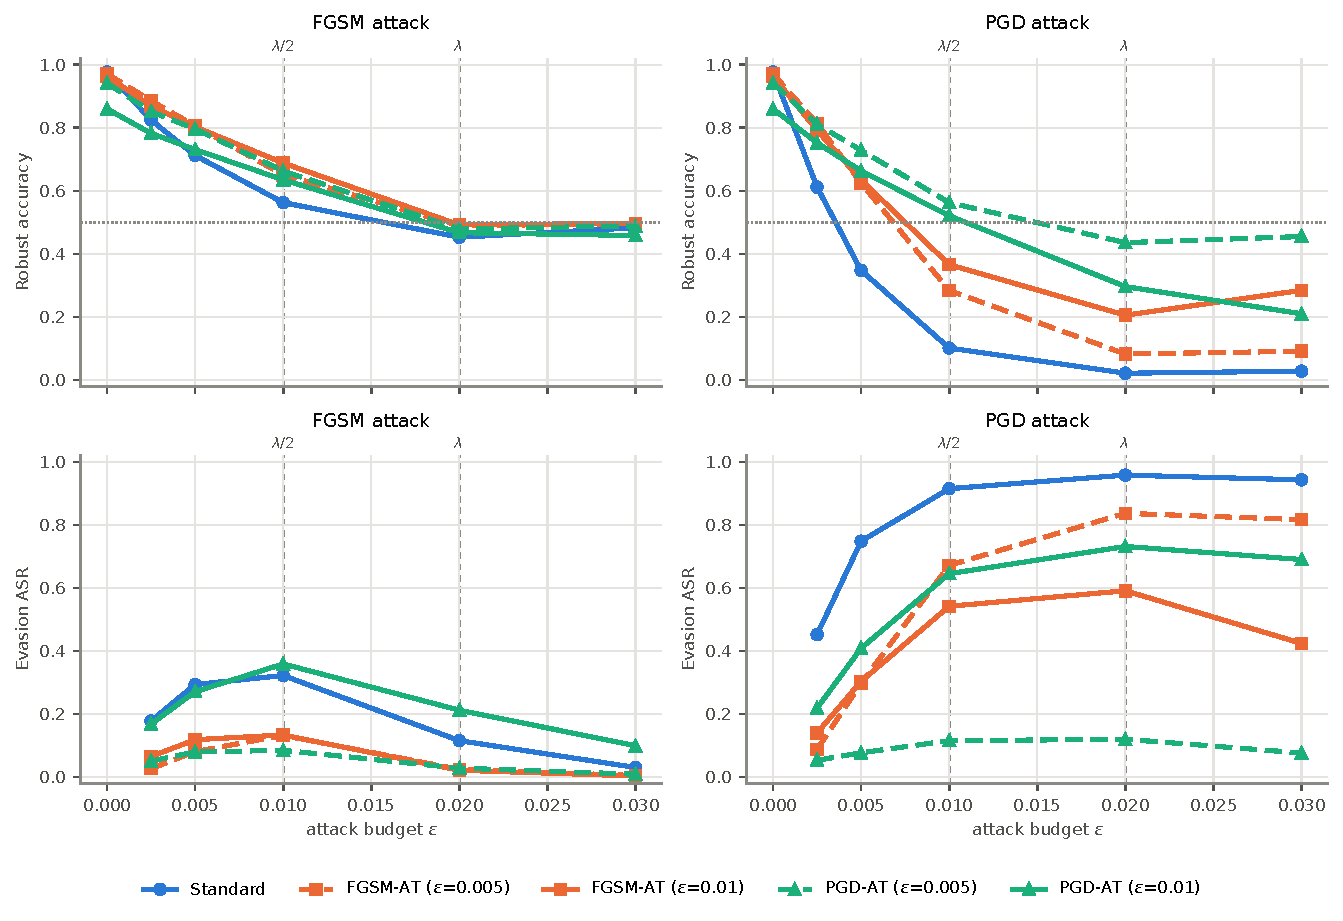
\includegraphics[width=0.8\textwidth]{figures/fig_h3_adv_training.pdf}}{\todo{figure}}
\caption{Standard vs.\ adversarially trained detectors ($\lambda=0.02$). Color: training method;
dashed: $\epsilon_{\text{train}}=0.005$, solid: $\epsilon_{\text{train}}=0.01$.}
\label{fig:advtrain}
\end{figure*}
\begin{table}[t]
\caption{Evasion attack success rate (\%) at $\lambda=0.02$; F = FGSM, P = PGD, column = attack $\epsilon$.}\label{tab:robust}
\small
\resizebox{\columnwidth}{!}{\IfFileExists{generated/table_robust.tex}{\begin{tabular}{lrrrrrr}
\toprule
Detector & F 0.005 & F 0.01 & F 0.02 & P 0.005 & P 0.01 & P 0.02 \\
\midrule
Standard & 29.4 & 32.2 & 11.6 & 74.9 & 91.5 & 95.8 \\
FGSM-AT ($\epsilon$=0.005) & 8.1 & 13.2 & 2.5 & 29.8 & 67.2 & 83.7 \\
FGSM-AT ($\epsilon$=0.01) & 11.9 & 13.4 & 2.2 & 30.4 & 54.2 & 59.1 \\
PGD-AT ($\epsilon$=0.005) & 8.0 & 8.5 & 2.8 & 7.7 & 11.6 & 12.0 \\
PGD-AT ($\epsilon$=0.01) & 27.1 & 35.9 & 21.2 & 40.9 & 64.6 & 73.2 \\
\bottomrule
\end{tabular}
}{\todo{table}}}
\end{table}
\textbf{Below $\lambda/2$, adversarial training works.} All four adversarially trained detectors
lower both attacks' evasion success for $\epsilon<\lambda/2$ (Figure~\ref{fig:advtrain},
Table~\ref{tab:robust}), at some cost in clean accuracy (Table~\ref{tab:clean}). The best is PGD
training at $\epsilon_{\text{train}}=0.005=\lambda/4$. Against PGD, its evasion success rate is
\PatAPgdAsrA\%, \PatAPgdAsrB\%, and \PatAPgdAsrC\% at $\epsilon=0.0025$, $0.005$, and $0.01$, versus
\BasePgdAsrA\%, \BasePgdAsrB\%, and \BasePgdAsrC\% for the standard detector; its accuracy under
PGD at $\epsilon=0.005$ is \PatAPgdAccB\% versus \BasePgdAccB\%. It gives up only
\BaseCleanAcc\,$\to$\,\PatACleanAcc\% clean accuracy.

\textbf{FGSM training mostly protects against FGSM.} FGSM-trained detectors resist FGSM well
(evasion success at most \FatBFgsmAsrC\% for $\epsilon\le\lambda/2$) but much less PGD (\FatAPgdAsrB\%
at $\epsilon=0.005$, versus \PatAPgdAsrB\% for the PGD-trained detector). They are still clearly
better than the standard detector, so this is not the complete ``catastrophic overfitting'' of
Wong et al.~\cite{wong2020fast}, but the same effect in milder form: robustness learned against a
single linear step only partly transfers to an iterative attack.

\textbf{Training at the limit backfires.} PGD training at $\epsilon_{\text{train}}=\lambda/2$ has
the lowest clean accuracy (\PatBCleanAcc\%, with TPR only \PatBCleanTpr\%) and is less robust than
PGD training at $\lambda/4$ at every attack budget. This is what Section~\ref{sec:limit} predicts:
at $\epsilon=\lambda/2$ every training pair has an adversarial point that would have to carry both
labels, so the training objective cannot be met.

\textbf{Beyond $\lambda/2$, apparent robustness is an artifact of the attack.} At large budgets the
PGD-trained detector ($\lambda/4$) still lets PGD evade only \PatAPgdAsrD\% of watermarks at
$\epsilon=\lambda$. The proposition says this cannot be real robustness, and the oracle attacker of
Table~\ref{tab:worst} confirms it: moving each image toward its counterpart, the oracle drives
\emph{every} detector to at most 50\% accuracy at $\epsilon=\lambda/2$ (PGD-trained: \PatAOracleAccC\%,
pairs both correct: \PatAOraclePairC\%), and at $\epsilon=\lambda$ it evades \PatAOracleAsrD\% of the
PGD-trained detector's detections by simply restoring the original image. PGD fails to find this
direction for the adversarially trained detectors, which is a reminder that a gradient attack only
gives an upper bound on robustness. Conversely, for small budgets PGD is far stronger than the
oracle (standard detector at $\epsilon=0.005$: \BasePgdAccB\% vs.\ \BaseOracleAccB\% accuracy),
because it exploits the detector's non-robust features rather than the watermark itself; a complete
evaluation needs both attacks.

\textbf{H3 holds for $\epsilon<\lambda/2$}, most strongly for PGD training at $\lambda/4$, and
fails, necessarily, at and above $\lambda/2$.

\begin{table}[t]
\caption{Accuracy (\%) under PGD and under the oracle attacker (Orc.), $\lambda=0.02$. At
$\epsilon=\lambda/2=0.01$ the oracle caps every detector at 50\%.}\label{tab:worst}
\small
\resizebox{\columnwidth}{!}{\IfFileExists{generated/table_worst.tex}{\begin{tabular}{lrrrrrr}
\toprule
Detector & \multicolumn{2}{c}{$\epsilon$=0.005} & \multicolumn{2}{c}{$\epsilon$=0.01} & \multicolumn{2}{c}{$\epsilon$=0.02} \\
 & PGD & Orc. & PGD & Orc. & PGD & Orc. \\
\midrule
Standard & 34.7 & 87.5 & 10.1 & 49.5 & 2.1 & 2.2 \\
FGSM-AT ($\epsilon$=0.005) & 62.4 & 91.2 & 28.4 & 49.4 & 8.2 & 2.9 \\
FGSM-AT ($\epsilon$=0.01) & 63.4 & 78.5 & 36.6 & 49.7 & 20.5 & 3.6 \\
PGD-AT ($\epsilon$=0.005) & 72.9 & 76.3 & 56.2 & 49.8 & 43.6 & 5.8 \\
PGD-AT ($\epsilon$=0.01) & 66.3 & 72.3 & 52.1 & 49.7 & 29.6 & 14.0 \\
\bottomrule
\end{tabular}
}{\todo{table}}}
\end{table}

\subsection{H4: Watermark strength}
\begin{figure*}[t]
\centering
\IfFileExists{figures/fig_h4_lambda.pdf}{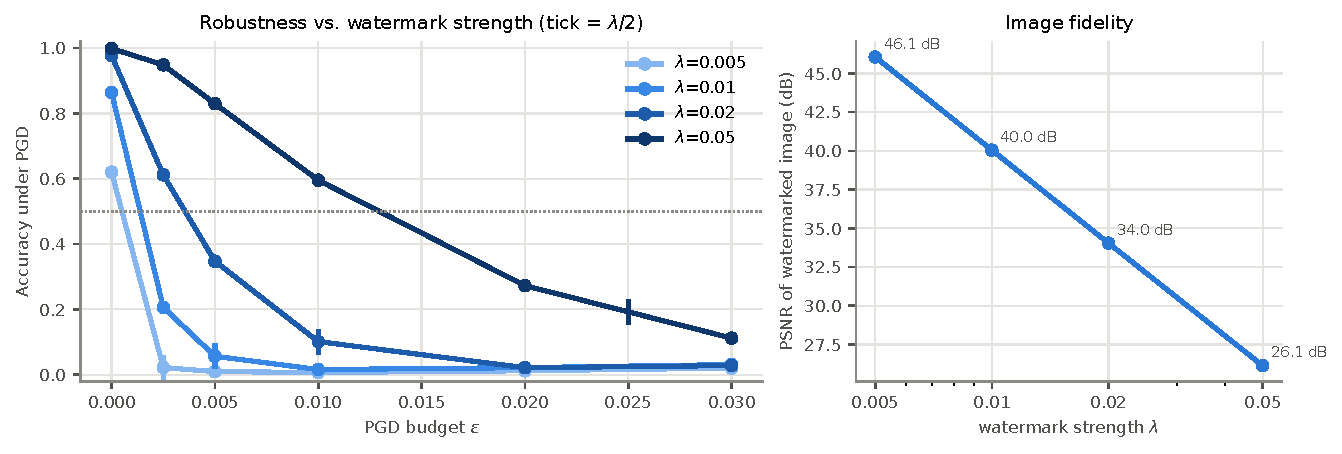
\includegraphics[width=0.85\textwidth]{figures/fig_h4_lambda.pdf}}{\todo{figure}}
\caption{Left: accuracy of standard detectors under PGD for each watermark strength; ticks mark each
$\lambda/2$. Right: fidelity of the watermarked image.}
\label{fig:lambda}
\end{figure*}
\begin{table}[t]
\caption{Watermark strength: fidelity and robustness (accuracy in \%, PGD).}\label{tab:lambda}
\small
\resizebox{\columnwidth}{!}{\IfFileExists{generated/table_lambda.tex}{\begin{tabular}{rrrrrrrr}
\toprule
$\lambda$ & PSNR & SSIM & Clean & P 0.0025 & P 0.005 & P 0.01 & P 0.02 \\
\midrule
0.005 & 46.1 & 0.997 & 62.0 & 2.2 & 0.9 & 0.7 & 1.2 \\
0.01 & 40.0 & 0.990 & 86.4 & 20.6 & 5.6 & 1.6 & 2.1 \\
0.02 & 34.0 & 0.963 & 97.7 & 61.2 & 34.7 & 10.1 & 2.1 \\
0.05 & 26.1 & 0.843 & 99.9 & 94.9 & 83.0 & 59.6 & 27.3 \\
\bottomrule
\end{tabular}
}{\todo{table}}}
\end{table}
A stronger watermark is more robust at every budget (Figure~\ref{fig:lambda},
Table~\ref{tab:lambda}). Under PGD at $\epsilon=0.005$, standard detectors keep
\LamAPgdAccB\%, \LamBPgdAccB\%, \BasePgdAccB\%, and \LamDPgdAccB\% accuracy for
$\lambda=0.005$, $0.01$, $0.02$, and $0.05$; at $\epsilon=0.01$ the strongest watermark still gives
\LamDPgdAccC\% while the others give at most \BasePgdAccC\%. Each curve collapses near its own
$\lambda/2$ (tick marks), as the proposition predicts. Clean detection also improves with $\lambda$,
from \LamACleanAcc\% to \LamDCleanAcc\%: the weakest watermark (about $1.3/255$ per pixel) is hard
to detect even without an attack. The price is fidelity: PSNR falls from \LamAWmPsnr\,dB to
\LamDWmPsnr\,dB (SSIM \LamAWmSsim\ to \LamDWmSsim), and at $\lambda=0.05$ the pattern is faintly
visible. \textbf{H4 holds}: robustness is bought directly with image quality.

\subsection{Cost of the attacks in image quality}
The attacks that defeat the standard detector are less visible than the watermark itself. The
watermark costs \BasePSNR\,dB PSNR. PGD at $\epsilon=0.0025$ changes the image by only
\BasePgdPsnrA\,dB and already evades \BasePgdAsrA\% of detections; at $\lambda/2$ it costs
\BasePgdPsnrC\,dB and evades \BasePgdAsrC\%. Figure~\ref{fig:examples} shows that the attacked
images are indistinguishable from the watermarked ones by eye. An attacker therefore does not
need to visibly damage an image to strip this watermark.
\begin{figure}[t]
\centering
\IfFileExists{figures/fig_examples.pdf}{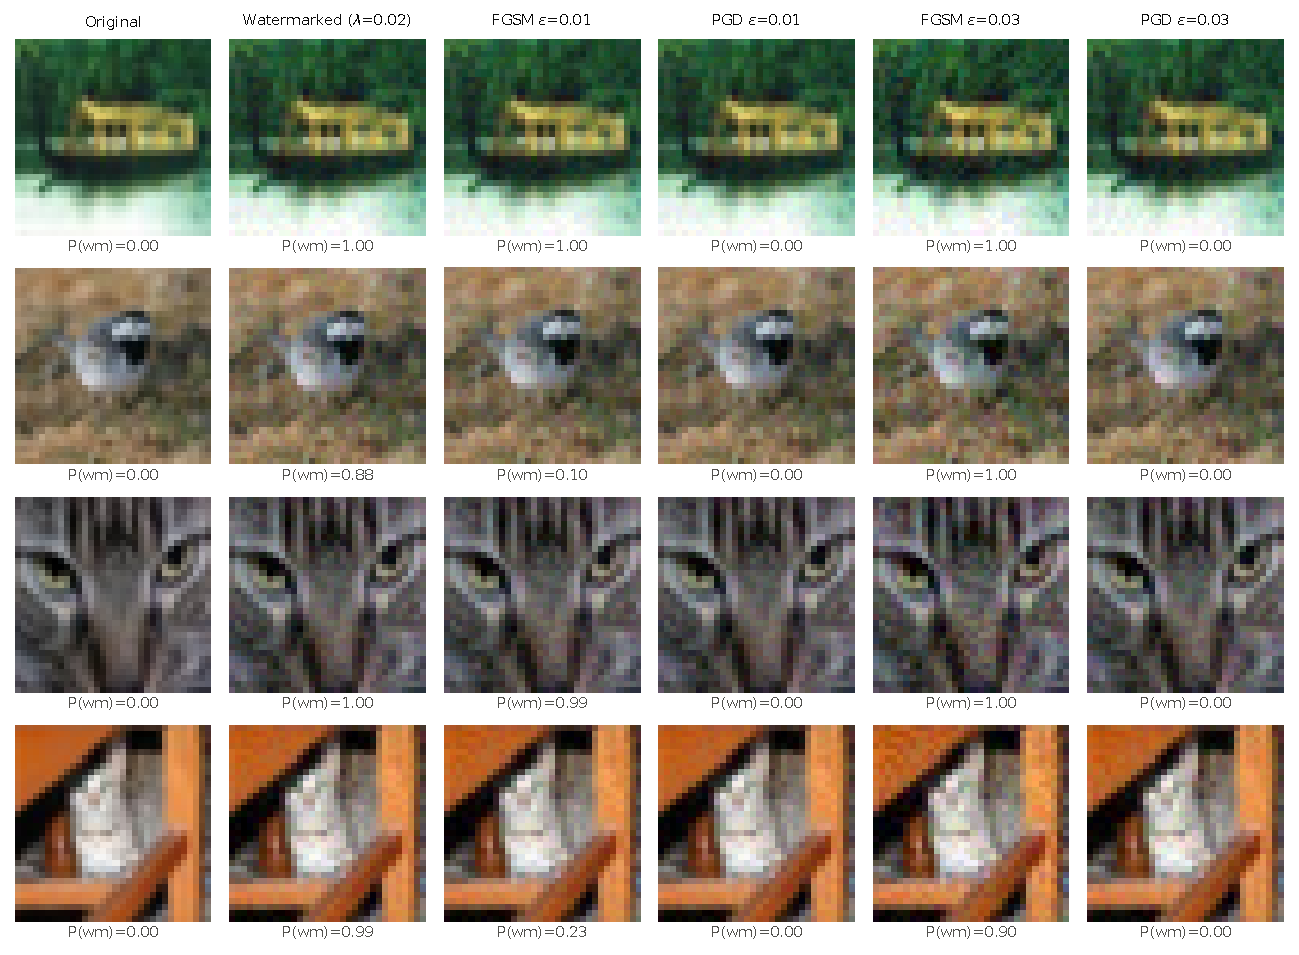
\includegraphics[width=\columnwidth]{figures/fig_examples.pdf}}{\todo{figure}}
\caption{Test images: original, watermarked, and attacked watermarked versions, with the
standard detector's probability that the image is watermarked.}
\label{fig:examples}
\end{figure}

\section{Discussion and Limitations}
\textbf{The watermark's amplitude is its security margin.} The proposition shows that, against
an $L_\infty$ attacker, the budget at which robust detection becomes impossible is fixed by the
watermark itself, not by the detector. Our results follow it closely: every detector collapses
near its $\lambda/2$, adversarial training helps only below it, training at it backfires, and the
oracle attacker reaches the bound exactly. Better detectors can approach the limit but not pass it;
the only lever beyond it is a larger $\lambda$, which costs fidelity (H4).

\textbf{The detector learns ``noise'', not only the key.} The random-noise control shows that the
standard detector flags clean images once they carry dense noise of amplitude near $\lambda$. A
learned detector trained only on clean vs.\ watermarked images has no reason to tell $W$ apart
from other high-frequency patterns, which makes it cheap to trigger false alarms. Training with
noisy negatives (clean images plus random noise, labelled clean) would be a natural fix, and so
would a non-learned correlation detector that tests specifically for $W$.

\textbf{Evaluating robustness needs more than one attack.} PGD overstated the robustness of the
adversarially trained detectors at large budgets, and the oracle understated the vulnerability of
the standard detector at small budgets. Reporting the worse of several attacks, including one built
from knowledge of the watermark, gives a far more honest picture than any single attack.

\textbf{Limitations.} The watermark is a fixed, additive, image-independent pattern, much simpler
than learned or diffusion-based watermarks~\cite{paper4,paper5,paper6}; such schemes have no
single amplitude, so our bound does not apply to them directly, although the same reasoning
applies to any watermark whose embedding changes each pixel by a bounded amount. The attacker is
white-box; black-box attackers are weaker. Images are $32\times32$, which is far smaller than real
generated images. We apply the watermark in floating point; with 8-bit storage, $\lambda=0.005$
(about $1.3/255$) would be partly erased by rounding. Each configuration was trained once (seed 0),
so small differences between models should not be over-interpreted.

\section{Conclusion}
A ResNet50 detector for a fixed invisible watermark is accurate on unmodified images but easy to
fool: PGD perturbations smaller than the watermark itself remove most detections (H1), and PGD is
consistently stronger than FGSM (H2), whose large steps instead add watermark-like noise.
Adversarial training, best with PGD at a budget of $\lambda/4$, makes the detector substantially
more robust, but only below $\lambda/2$ (H3). Beyond that point no detector can be robust, because
the clean and watermarked versions of an image are within reach of a common point; only a stronger
watermark moves the limit, at a direct cost in image quality (H4).

\noindent\textbf{Contributions.} All six authors contributed equally to this project.

\noindent\textbf{AI usage.} The proposal was edited with assistance from ChatGPT. Parts of the
team's exploratory notebook were written with assistance from ChatGPT. The final experiment code
(\texttt{wmrobust.py}, \texttt{run\_experiments.py}, \texttt{make\_report\_assets.py}), the final
notebook, and drafts of this report were written with assistance from Claude (Anthropic) and
reviewed by the team.

\nocite{*}
\bibliographystyle{ACM-Reference-Format}
\bibliography{reference}

\end{document}
\endinput
